\chapter{IMPLEMENTATION}

\section{Hardware}

\hspace{0.9cm} The main system has i7, 6700k processor with 16gb DDR4 RAM clocked at 2133MHz.
Graphics Processing Unit (GPU) which is Nvidia Titan X (Maxwell Gen.) 12gb GDDR5 VRAM. This particular system was running Windows 10 Pro x64 build 1607.
For the sake of comparison we implemented the project on MacBook Air 13 inch early 2015 edition with specs of intel core i5 at 1.6kHz and 4gb DDR 3 1600MHz.
This particular system did not possess a discrete GPU.
Therefore it provided a good benchmark analysis of a graphics enabled version vs CPU only version of the project.
MacBook Air was running MacOS sierra as the operating system.
\begin{table}[]
	\centering
	\caption{SYSTEM CONFIGURATION FOR EXPERMIENTAL SYSTEMS}
	\label{table-1}
	\vspace{0.9cm}
	\begin{tabular}{|l|l|l|l|l|}
		\hline
		Processor                                                                 & \begin{tabular}[c]{@{}l@{}}Physical\\ RAM\end{tabular}                                    & \begin{tabular}[c]{@{}l@{}}CUDA\\ GPU name\end{tabular}                                           & \begin{tabular}[c]{@{}l@{}}MATLAB\\ GPU support\end{tabular} & \begin{tabular}[c]{@{}l@{}}Operating system\\ and build\end{tabular}                                                  \\ \hline
		\begin{tabular}[c]{@{}l@{}}Intel\\ Core i7\\ 6700k @\\ 4 GHz\end{tabular} & \begin{tabular}[c]{@{}l@{}}2 × 8 GB\\ Kingston\\ DDR4 Non\\ ECC @\\ 2133 MHz\end{tabular} & \begin{tabular}[c]{@{}l@{}}NVIDIA\\ Titan X\\ Maxwell\\ Architecture\\ 12 GB\\ GDDR5\end{tabular} & Yes                                                          & \begin{tabular}[c]{@{}l@{}}Windows 10\\ 64 bit Build 1607,\\ Custom PC Build\end{tabular}                             \\ \hline
		\begin{tabular}[c]{@{}l@{}}Intel\\ Core\\ i5 @\\ 1.6 GHz\end{tabular}     & \begin{tabular}[c]{@{}l@{}}4 GB\\ DDR3 Non\\ ECC @\\ 1600 MHz\end{tabular}                & N/A                                                                                               & No                                                           & \begin{tabular}[c]{@{}l@{}}MacOS Sierra\\ 10.12.2 Build\\ 16C67 on\\ MacBook Air\\ Early 2015,\\ 13 inch\end{tabular} \\ \hline
	\end{tabular}
\end{table}


\section{Software}

\hspace{0.9cm} Matlab was chosen as the software to build the project. Dealing with large amounts of data meant that we needed a quick way to evaluate results and import and export data conveniently. All these features were readily made available by Matlab and hence it was the ideal software for completing the project.The GPU acceleration provided by Matlab is through the CUDA runtime which is transparently available to the programs with only slight modifications required for GPU based code.
\\
The following steps are taken in software to execute the project:\\
\begin{enumerate}
	\item Import data from the data source.
	\item Run transformation of the dataset to an image.
	\item Feed generated image into the neural network generated by Matlab.
\end{enumerate}

\begin{figure}[h!]
	\centering	
	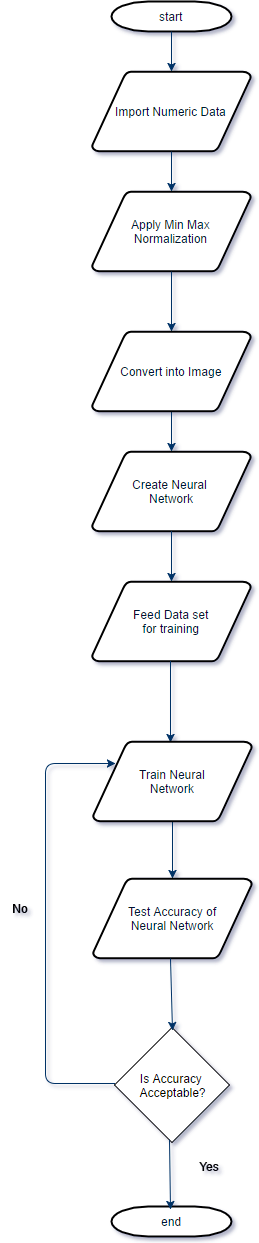
\includegraphics[width=1.5in]{Flowchart.png} % e.g. insert ./image for image.png in the working directory, adjust scale as necessary
	\caption{ Flowchart.}
	\label{fig:9} % insert suitable label, this is used to refer to a fig from within the text as shown above
	
\end{figure}
\section{Algorithm}
Raw numeric data is first transformed into the grey
scale color domain via min-max normalization. Min-max
normalization preserves the integrity of data via scaling.
Various methods exist for normalization [10], but the proposed
method requires scaling to an interval between [0, 255] hence,
we use min-max normalization. Eq. 1 describes min-max
normalization, which is a step in the proposed method.
\begin{equation} X'=a+ \frac{(X- X_{min})(b-a)}{X_{max} - X_{min}} \end{equation}.
	

Here, X is the normalized pixel. X is the current pixel in
consideration. X\textsubscript{max} and X\textsubscript{min} is the maximum and minimum
value of the dataset respectively, a and b are the minimum and
maximum values of the color space. Since, the color space is
8 bit we scale the dataset to the interval [0, 255] where a is 0
and b is 255. Hence, we get the following equation:-
\begin{equation} X'=a+ \frac{(X- X_{min})255}{X_{max} - X_{min}} \end{equation}.
Thus, we get the dataset normalized into the greyscale color
space. We, then convert the processed data set into images
depending on the time scale. Eq. 3.2 provides us with a direct
formula for converting textual data into a grayscale image.\\
The results of the above described process is given in the next section.